\subsubsection{Dimensionamento da base}

Para manipuladores com longo alcance, as forças e torques envolvidos requerem
uma estrutura de fixação do robô de forma que o sistema como um todo não se
movimente e, no caso extremo, tombe. Normalmente, os manipuladores robóticos são
fixados no chão e as características da superfície e tamanho dos parafusos
necessários são estipulados pelo fornecedor a partir dos valores máximos de
torque e força que o manipulador pode exercer em seu ponto de apoio.
Considerando um manipulador centrado em uma base circular apoiada no chão, dois
fatores influenciam capacidade de estabilização da estrutura: o raio da base e o seu peso.

O raio da base $r_{b}$ é limitado pelo ambiente da turbina e para cada escolha
de posicionamento existem restrições específicas. 
Para a realização dos cálculos de dimensionamento foi considerado,
primeiramente, o manipulador posicionado em frente a pá, como ilustrado na
figura \ref{fig::robot_front}.

\begin{figure}[H]
\centering
	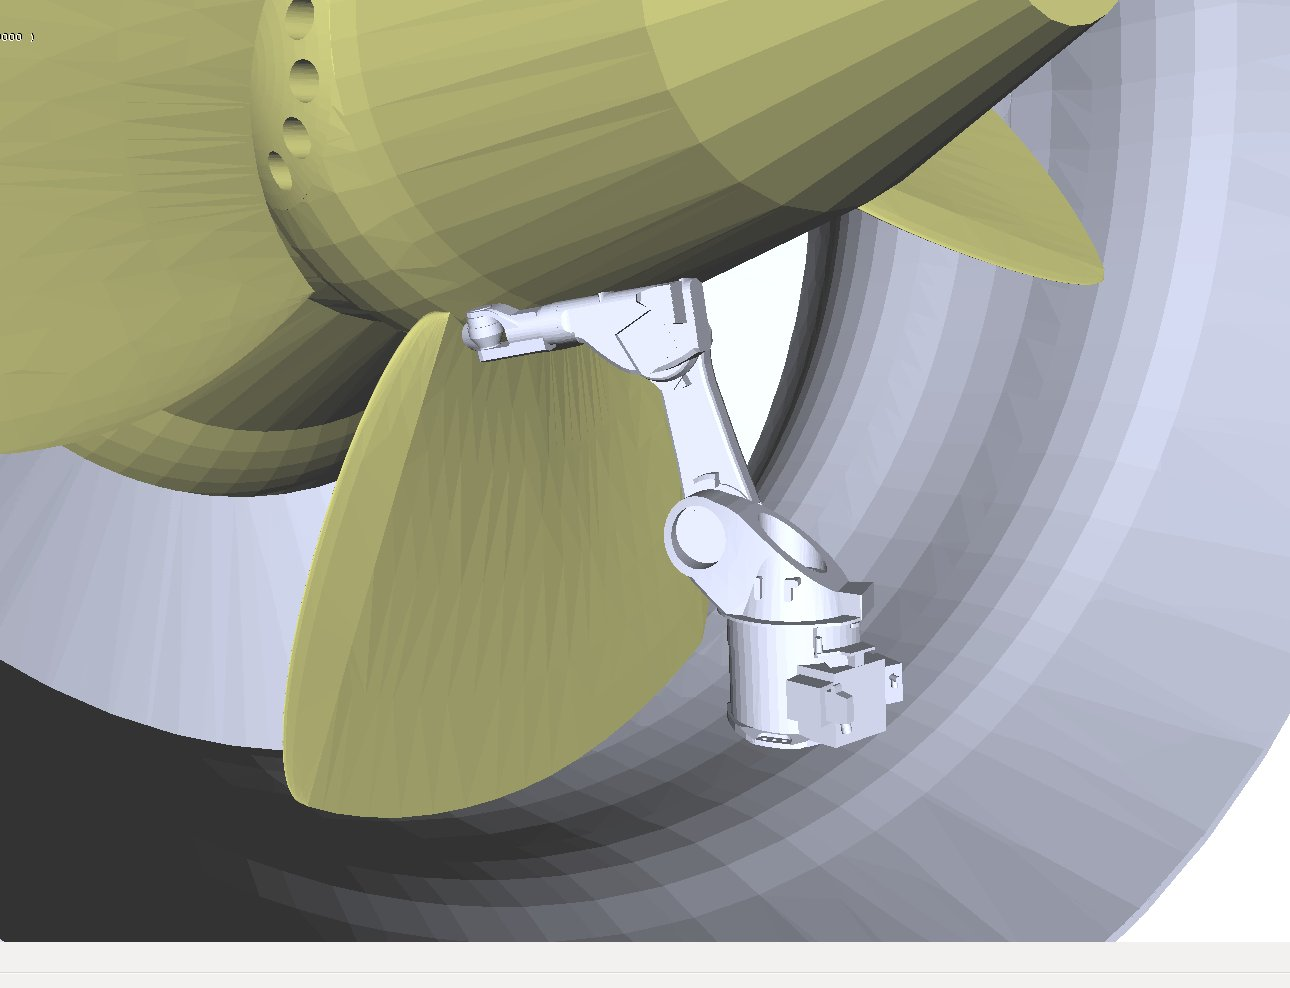
\includegraphics[width=0.7\columnwidth]{sota/figs/openrave/robot_front_openrave.jpg}
	\caption{Exemplo de posicionamento de um manipulador robótico em frente à pá.}
	\label{fig::robot_front}
\end{figure}

 %TODO figura robo na frente da turbina
Nessa posição é possivel processar uma face por
vez, a uma altura de 1000mm do chão, com um alcance mínimo do manipulador de
1800mm.
Para essa
configuração, a tamanho máximo no sentido perpendicular ao fluxo d'água que
a base pode assumir é de aproximadamente 1600mm. Existe ainda a curvatura do aro
câmara e a estrutura deve ser projetada de forma a seguir os
contornos impostos pelo ambiente.
A figura \ref{fig::base_aro_frente} 
representa um esboço da vista frontal do aro câmara e a largura máxima que a
base pode assumir. A análise da dimensão máxima da base no sentido paralelo ao
fluxo d'água pode ser realizada com o auxílio do desenho técnico fornecido pela
ESBR, ilustrado na figura \ref{fig::turbine_side}.

\begin{figure}[H]
\centering
	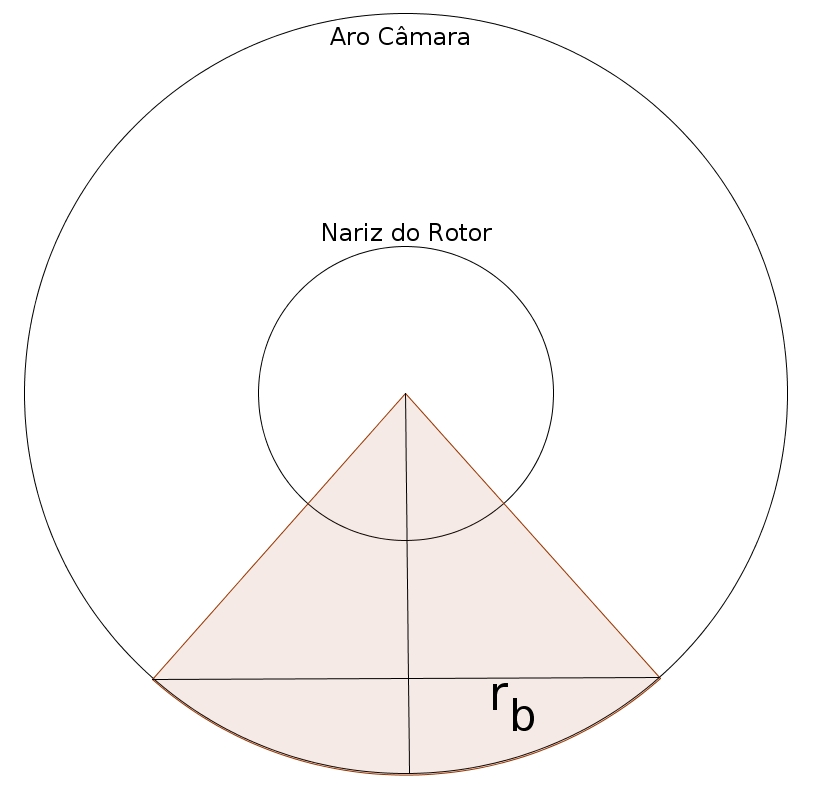
\includegraphics[width=0.7\columnwidth]{sota/figs/base/base_aro_frente.jpg}
	\caption{Visão frontal do aro câmara e raio máximo da base.}
	\label{fig::base_aro_frente}
\end{figure}

O limite superior do raio da base nessa
região é determinado pela região de transição do aro câmara para o tubo de
descarga, onde há uma mudança na inclinação do plano de apoio. A região,
considerada horizontal, que pode acomodar a base do manipulador tem um
comprimento de aproximadamente 1400mm no sentido do fluxo do rio.
Entrentanto, esse limite pode ser contornado construindo-se um plano de apoio
horizontal ou projetando-se a base de forma que ela acompanhe essa
inclinação.É necessário, então, considerar o dimensionamento da base no
cálculo do alcance mínimo do manipulador,que agora se encontra deslocado em
relação à superfície da pá. Sendo assim, alcance mínimo se relaciona com o tamanho do raio da base de 
acordo com $$a_{min}=\sqrt{r_b^2+1800^2}.$$

\begin{figure}[H]
\centering
	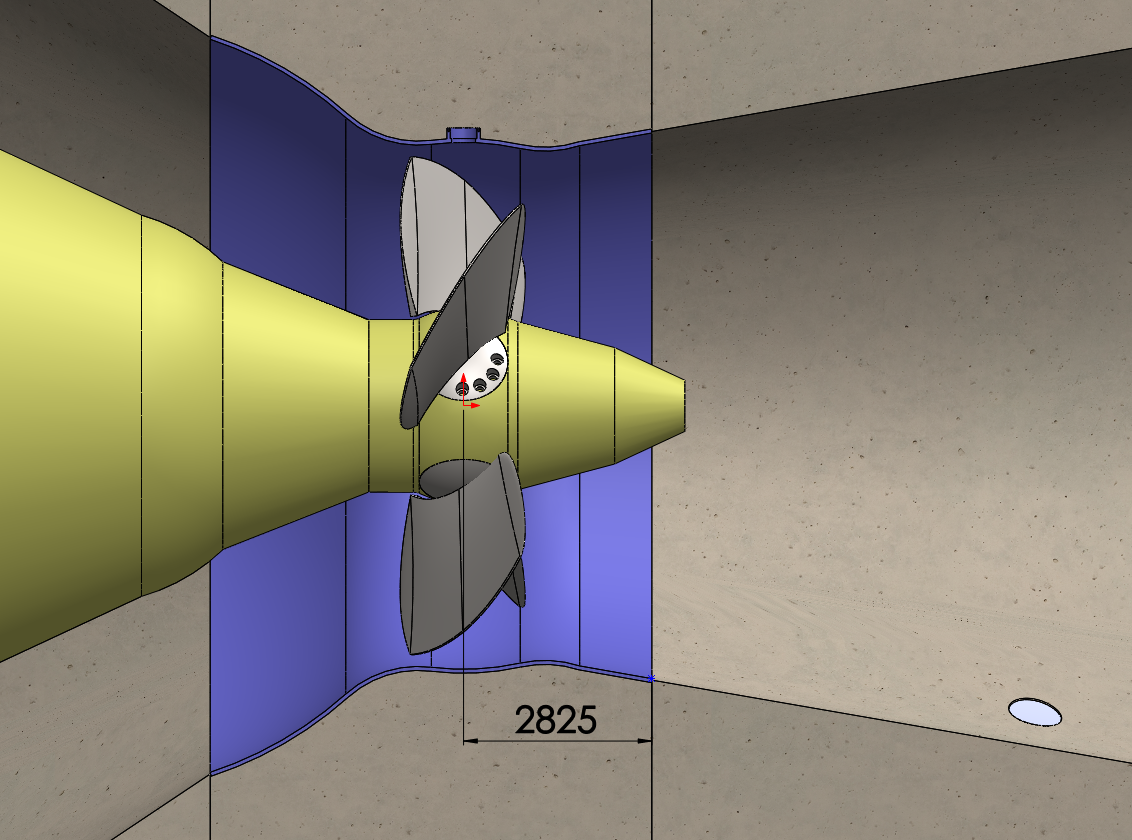
\includegraphics[width=0.7\columnwidth]{sota/figs/base/turbine_side}
	\caption{Visão lateral do aro câmara e raio máximo da base nessa direção.}
	\label{fig::turbine_side}
\end{figure}



% \begin{figure}[H]
% \centering
% 	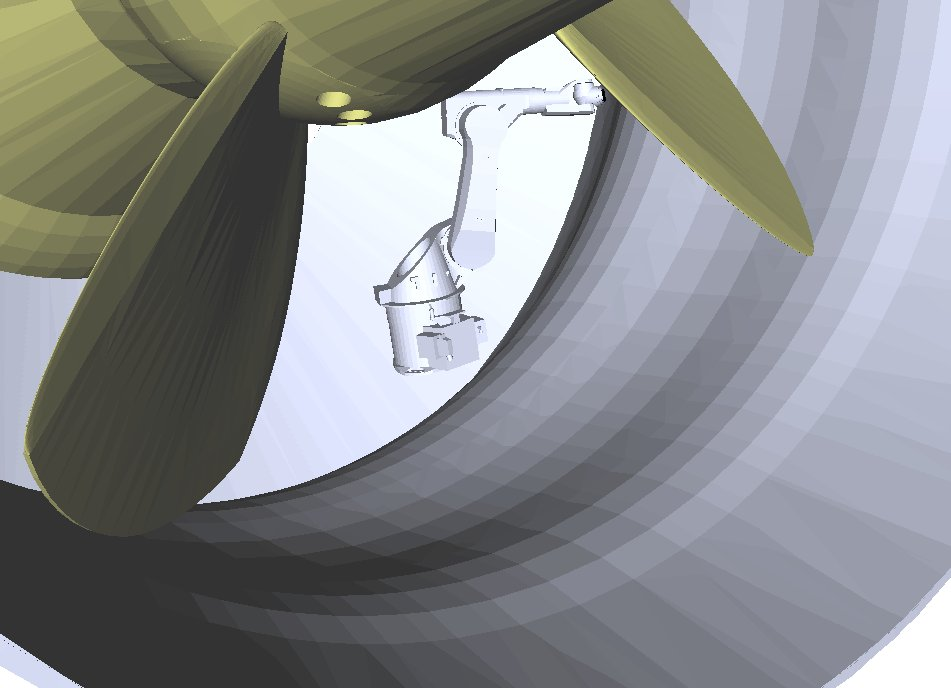
\includegraphics[width=0.7\columnwidth]{sota/figs/openrave/robot_between_openrave.jpg}
% 	\caption{Exemplo de posicionamento de um manipulador robótico entre as pás.}
% 	\label{fig::robot_between}
% \end{figure
O cálculo das dimensões da base com o robô posicionado dentro do aro câmara e
entre as pás depende do
ângulo de ataque das pás. A distância entre as pás pode ser calculada por meio
do cálculo do ângulo diédrico,definido como o espaço entre dois semiplanos não contidos num mesmo
plano com origem numa aresta comum, entre elas. A amplitude do movimento de
rotação $alpha$ das pás é de $14,5^o$ para cada lado a partir da posição zero,
entretanto \textbf{essa posição não pôde ser informada no momento da viagem de
reconhecimento e ainda não foi disponibilizada}. Para critério de cálculos foi
utilizado um ângulo de $45^o$ como a posição de maior abertura das pás e o zero
foi considerado como a reta perpendicular ao fluxo de água. O ângulo diédrico
$\theta$ entre as pás depende do ângulo de ataque das pás e obedece a relação
$\cos{\theta} = \sin^2{\alpha}.$

O a distância entre as pás, considerada como o arco de circunferência no aro
câmara descrito pelo ângulo diédrico calculado, pode ser obtido a partir da
relação $arc=R\alpha$.
Considerando o raio do aro do câmara comoo R=3850mm, o raio máximo da base pode
ser calculado como $$r_{b_e} = (R - h_{b_e})\tan{\theta/2}$$ e com $h_{b_e}$
sendo a altura da base.

O peso mínimo que a base do robô deve possuir está diretamente relacionada com o
tamanho de seu raio. A firgura \ref{fig::tilt_robot} faz uma representação
simplificada da forma que o torque de capotamento máximo atua no robô e em sua
base. Na situação limite, considerando um torque com sentido horário, a força
normal entre a base e a superfície de apoio, $N_2$, teria módulo igual a zero.
No pior caso, podemos considerar que a força vertical exercida pelo robô em sua
base é composta apenas pelo seu peso $W$ e, para que a base não se mova, o
somatório das forças e torques devem ser iguais a zero.

A análise do somatório das forças nos fornece a relação $N_1=W$  e o somatório
dos torques se reduz a $M_k-Wr_b=0$. Sendo assim, a relação entre o raio da base, seu 
peso e o torque máximo de capotamento exercido pelo robô é
da forma 

$$M_k=Wr_b.$$

%TODO refazer figura
\begin{figure}[H]
\centering
	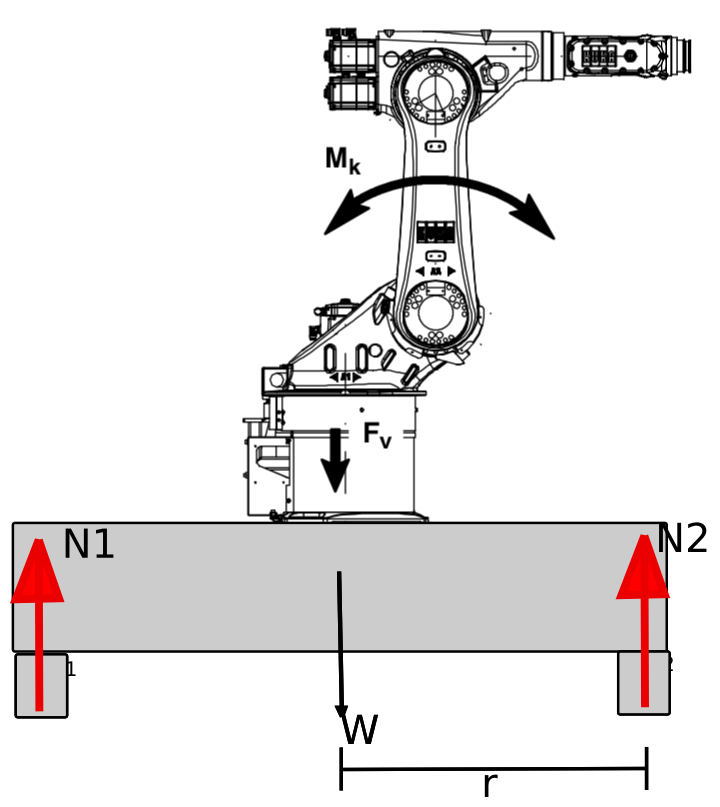
\includegraphics[width=0.6\columnwidth]{sota/figs/base/tilt}
	\caption{Forças e torques máximos entre o robô e sua base.}
	\label{fig::tilt_robot}
\end{figure}

%TODO comparativo entre raio e peso

Uma vez que a superfície do aro câmara e a região adjacente no tubo de sucção
são \textbf{ferromagnéticas}, é possível a utilização de bases magnéticas para
uma compensação do peso e raio necessários para a estabilização do robô. Os
dispositivos magnéticos se dispõem de duas em duas principais catergorias para
essa aplicação:
dispositivos eletretromagnéticos e de imãs permanentes. O primeiro caso tem como
principal vantagem a possibilidade de acionamento remoto, entretanto para situações de
falha em que haja perda de fornecimento de energia, a força de atração também é
perdida. O segundo caso consiste em imãs permanentes arrumados de maneira que
seja possível organizar o seu fluxo magnético e, assim, controlar por meio de
uma alavanca a presença ou ausência de força magnética. A figura
\ref{fig::base::imas} ilustra os dois tipos de bases magnéticas citados.

\begin{figure}[H]
\begin{subfigure}[b]{0.5\columnwidth}
  \centering
  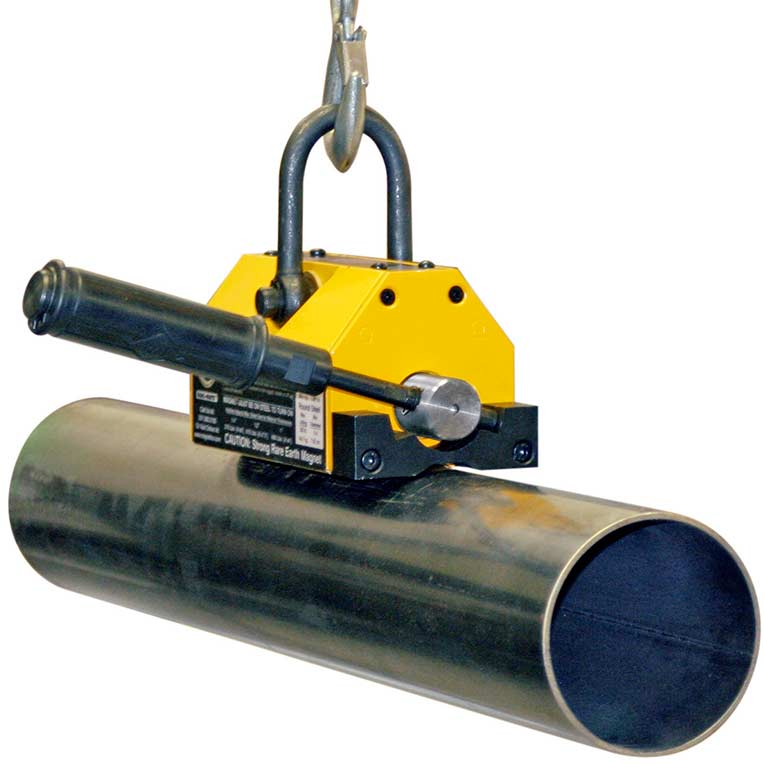
\includegraphics[width=.7\columnwidth]{sota/figs/base/mangnetpipe}
  \caption{Tipo imã permanente}
  \label{fig:sfig1}
\end{subfigure}%
\begin{subfigure}[b]{0.4\columnwidth}
  \centering
  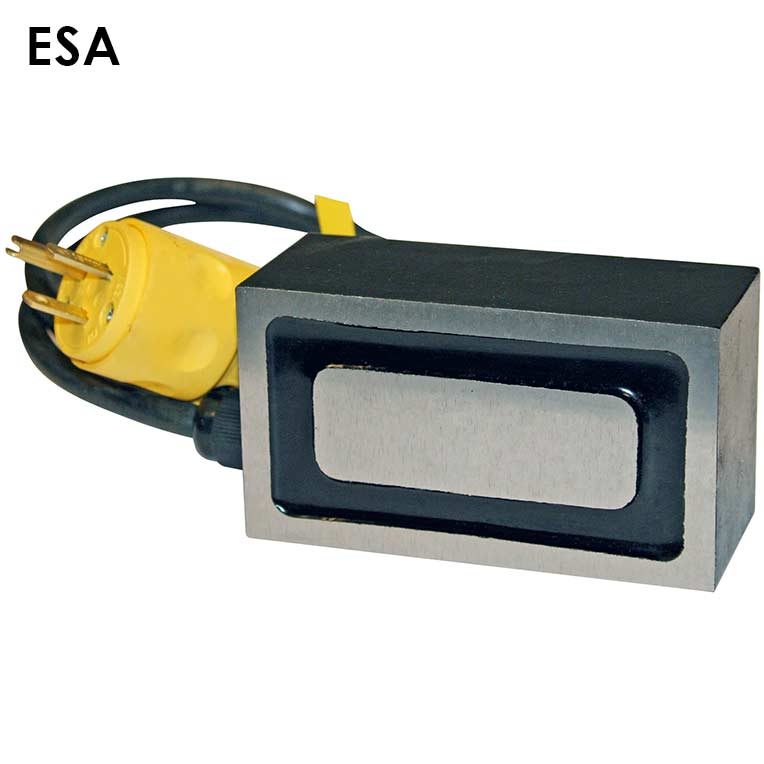
\includegraphics[width=.7\columnwidth]{sota/figs/base/eletromagnet}
  \caption{Tipo eletroimã}
  \label{fig:sfig2}
\end{subfigure}
\caption{Tipos de bases magnéticas comerciais.}
\label{fig::base::imas}
\end{figure}

Comercialmente, foram encontrados bases magnéticas com capacidade de até 3000N.
Um dos requerimentos para a utilização de bases magnéticas, sejam
eletromagnéticas e de imãs permanentes, é a limpeza da superfície de contato
para um acoplamento efeiciente. Essa restrição força a presença humana para a
limpeza e, sobretudo, a verificação de uma correta fixação. Sendo assim, as
bases magnéticas de imã permanente se mostram mais coerentes para a aplicação,
pois não possuem ponto de falha para o caso de perda de energia do sistema e
possuem uma maior capacidade de carga. A curvatura do ambiente não é um
limitante, sendo possível até a confecção de uma máscara para a base de maneira
que a superfície de apoio se conforme perfeitamente com a superfície de fixação.
